%% LyX 1.6.5 created this file.  For more info, see http://www.lyx.org/.
%% Do not edit unless you really know what you are doing.
\documentclass[spanish]{scrreprt}
\usepackage[T1]{fontenc}
\usepackage[latin9]{inputenc}
\setcounter{secnumdepth}{3}
\setcounter{tocdepth}{3}
\usepackage{amsmath}
\usepackage{graphicx}
\usepackage{babel}
\addto\shorthandsspanish{\spanishdeactivate{~<>}}

\begin{document}

\title{Transcripcion\\
Notas de la Tesis\\
1er Reuni�n}


\date{05/04/2011}

\maketitle

\chapter*{Introduccion}

En esta reuni�n nos dedicamos a explorar distintas t�cnicas y herramientas
con las que modelar el problema de los efectos de la variaci�n de
la temperatura sobre el comportamiento de la estructura secundaria
del RNA del virus Junin, con las cuales se desarrollar�a un sistema
que deber�a arribar a las conclusiones ya obtenidas.

Se investigo cual seria la informaci�n que deber�a otorg�ndole a la
base de conocimiento como definiciones y reglas que el sistema tendr�a
para deducir. Tambi�n se discuti� la necesidad de especificarle al
sistema una meta o pregunta a responder. Por ultimo se buscaron las
herramientas necesarias para desarrollar dicho sistema y se discuti�
cual seria la dimensi�n del proyecto con las herramientas que fue
planteado.


\chapter*{Definiciones y Reglas}

Las definiciones que contendr�a la base para el proceso deductivo
serian las siguientes:
\begin{itemize}
\item $S^{+}\equiv"Se\, produce\, RNA\, genomico"$
\item $S^{-}\equiv"Se\, produce\, RNA\, antigenomico"$
\item $NP\equiv"Se\, produce\, nucleoproteina"$
\item $GPC\equiv"Se\, produce\, glicoproteina"$
\item $loop\_chico\equiv"La\, zona\, intergenica\, es\, achatada"$
\item $\neg loop\_chico\equiv"La\, zona\, intergenica\, es\, normal"$
\item $lectura\_completa\equiv"El\, RNA\, se\, puede\, leer\, completo\, sin\, cortes"$
\item $\neg lectura\_completa\equiv"El\, RNA\, no\, se\, puede\, leer\, completo\, sin\, cortes"$
\item $T\equiv"Aumenta\, la\, temperatura"$
\item $\neg T\equiv"Disminuye\, la\, temperatura"$
\end{itemize}
Utilizando estas definiciones , agregaremos las siguientes reglas:
\begin{itemize}
\item $S^{+}\,\wedge\, T\,\implies\, x(S^{+}\,\wedge\, loop\_chico)$
\item $S^{-}\,\wedge\, T\,\implies\, x(S^{-}\,\wedge\,\neg loop\_chico)$
\item $S^{+}\,\wedge\, loop\_chico\,\implies\, x(S^{+}\,\wedge\, lectura\, completa)$
\item $S^{+}\,\wedge\,\neg loop\_chico\,\implies\, x(S^{+}\,\wedge\,\neg lectura\, completa)$
\item $S^{-}\,\wedge\, loop\_chico\,\implies\, x(S^{-}\,\wedge\, lectura\, completa)$
\item $S^{-}\,\wedge\,\neg loop\_chico\,\implies\, x(S^{-}\,\wedge\,\neg lectura\, completa)$
\item $S^{+}\,\wedge\, lectura\, completa\,\implies\, x(S^{-}\,\wedge\,\neg S^{+})$
\item $S^{+}\,\wedge\,\neg lectura\, completa\,\implies\, x(NP\,\wedge\,\neg S^{+})$
\item $S^{-}\,\wedge\, lectura\, completa\,\implies\, x(S^{+}\,\wedge\,\neg S^{-})$
\item $S^{-}\,\wedge\,\neg lectura\, completa\,\implies\, x(GPCP\,\wedge\,\neg S^{-})$
\item $T\,\implies\, x(T)$
\item $S^{+}\,\wedge\,\neg T\,\implies\, x(NP\,\wedge\,\neg S^{+})$
\item $S^{-}\,\wedge\,\neg T\,\implies\, x(GPCP\,\wedge\,\neg S^{-})$%
\footnote{Este lo agregue yo, no estoy seguro si estar�a bien.%
}
\end{itemize}
El operador $\neg$ es utilizado como supresor%
\footnote{Si mal no recuerdo solo val�a para los RNA y para el Loop pero no
para $lectura\_completa$.%
} , por ejemplo en el caso de $S^{+}$ cuando aparece $\neg S^{+}$estos
se cancelan.


\chapter*{Metas Vs Goalless Planning}

En la discusi�n se planteo la dificultad que tiene el saber que pregunta
realizarle al sistema , osea en $A\,\implies\, B$ cual seria el $A$
desde el cual queremos partir y a que $B$ queremos llegar. 

Si bien el $A$ es mas f�cil de definir el $B$ supone un gran inc�gnita
en algunos casos , adem�s seria �til el poder averiguar otras posibles
conclusiones que se puedan derivar desde $A$ con lo contenido en
la base de conocimientos. Por esta raz�n se decidi� que lo mejor seria
no definir una meta (el $B$).

A causa de este cambio de estrategia y de el hecho de que requerimos
realizar cambios de estado%
\footnote{La eliminaci�n u conversi�n de los RNA a prote�nas u sus complementos
, los cambios de temperatura y el tama�o del loop requieren poder
ser modificados duramente el proceso, cosa que DL no puede hacer por
si solo.%
} se propusieron 2 estrategias posibles , Planning y L�gicas Temporales.
A estas 2 propuestas se las fusiono de la siguiente manera :\\


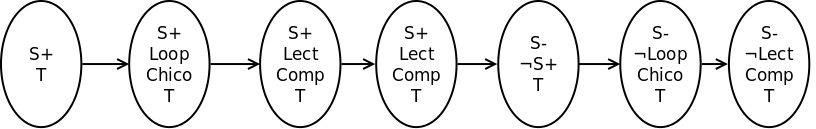
\includegraphics[clip,width=0.8\textwidth,height=0.8\textheight,keepaspectratio]{ejemplo_planning}\\
Entre cada transicion el sistema de planning puede consultar a
la base de conocimiento para buscar otras \emph{interpretaciones equivalentes}%
\footnote{Me refiero a que en la base de conocimiento podriamos re interpretar
$loop\_chico$ como $lectura\_completa$ gracias a las reglas que
la base provee y lo mismo seria para el uso de definiciones y conceptos.%
}\emph{ }con las cuales arribar a nuevas conclusiones. Una conclusion
final seria la que se obtiene al no poder avanzar mas en una rama
del arbol de planeamiento ni siquiera recurriendo a nueva interpretaciones
de dicho estado.


\chapter*{Herramientas}

Quedo definido que se utilizara Racer 2.0 , salvo que se encuentre
alguna alternativa en Software Libre con prestaciones similares. 

No quedo muy en claro%
\footnote{Al menos para mi :\$.%
} en que lenguaje se implementaria lo relacionado con DL , pero se
decidio que se podria buscar alguna base de conocimiento que se adaptara
a esto o sino un sistema generico que ademas nos proveyera con un
lenguaje para agregar las reglas , conceptos y operadores para manipularlo. 

Debemos recordar que al ser un Planning Goalless no perdemos la propiedad
favorable de \emph{seudo-polinomial} que tienen los sistemas de planning
, asi que la eficiencia no seria algo tener en cuenta a la hora de
implementarlo.
\end{document}
